\section{Análisis de Costos del Prototipo}

El desarrollo del kit de clasificación requirió inversión en materiales de fabricación, componentes electrónicos comerciales, y herramientas especializadas. Este análisis desglosa los costos de prototipado considerando tanto la fabricación de una unidad individual como la producción de múltiples kits para uso en laboratorio.

\subsection{Estructura de Costos}

Los costos del proyecto se organizan en tres categorías principales: materiales mecánicos y de fabricación, componentes electrónicos y de control, y herramientas de fabricación que representan inversión de capital reutilizable.

\subsubsection{Materiales Mecánicos y de Fabricación}

La Tabla \ref{tab:materiales_kit} presenta el desglose detallado de materiales requeridos para fabricar un kit completo, incluyendo componentes fabricados (FDM, corte láser) y componentes comerciales (tornillería, contenedor, bomba de vacío).

\begin{table}[H]
\centering
\caption{Materiales y componentes para fabricación de un kit}
\label{tab:materiales_kit}
\footnotesize
\begin{tabular}{|l|c|r|r|}
\hline
\textbf{Producto} & \textbf{Cant.} & \textbf{Costo Unit. (COP)} & \textbf{Costo Total (COP)} \\
\hline
\multicolumn{4}{|l|}{\textit{Materiales de impresión 3D}} \\
\hline
Filamento varios tipos (kg) & 1.5 & 90,000 & 135,000 \\
\hline
\multicolumn{4}{|l|}{\textit{Insertos roscados}} \\
\hline
Insertos M3 para plástico & 20 & 300 & 6,000 \\
Insertos M4 para plástico & 4 & 400 & 1,600 \\
Insertos M4 para madera & 20 & 500 & 10,000 \\
\hline
\multicolumn{4}{|l|}{\textit{Tornillería}} \\
\hline
Tornillos M3 × 12 mm & 1 & 200 & 200 \\
Tornillos M3 × 16 mm & 1 & 250 & 250 \\
Tornillos M3 × 20 mm & 24 & 300 & 7,200 \\
Tornillos M3 × 25 mm & 2 & 350 & 700 \\
Tornillos M4 × 20 mm & 8 & 350 & 2,800 \\
Tornillos M4 × 30 mm & 4 & 400 & 1,600 \\
Tornillos M8 × 25 mm & 4 & 400 & 1,600 \\
Tornillos M10 × 35 mm & 4 & 500 & 2,000 \\
Tuercas M3 & 26 & 100 & 2,600 \\
Tuercas M4 & 4 & 400 & 1,600 \\
Tuercas M8 & 4 & 400 & 1,600 \\
Tuercas M10 & 4 & 500 & 2,000 \\
\hline
\multicolumn{4}{|l|}{\textit{Materiales estructurales}} \\
\hline
Cable Molex (metro) & 1 & 1,600 & 1,600 \\
Espuma (m²) & 1 & 2,500 & 2,500 \\
Amarres plásticos cortos & 4 & 200 & 800 \\
Tubo ovalado closet (6m) & 0.7 & 3,400 & 2,380 \\
Corte láser MDF 9mm & 1 & 27,000 & 27,000 \\
\hline
\multicolumn{4}{|l|}{\textit{Acabados}} \\
\hline
Sellador (galón) & 0.2 & 80,000 & 16,000 \\
Laca (galón) & 0.2 & 80,000 & 16,000 \\
Lijas (varias) & 1 & 5,000 & 5,000 \\
\hline
\multicolumn{4}{|l|}{\textit{Contenedor y accesorios}} \\
\hline
Canastilla plástica & 1 & 15,000 & 15,000 \\
Tapa canastilla plástica & 1 & 10,000 & 10,000 \\
\hline
\multicolumn{4}{|l|}{\textit{Sistema neumático}} \\
\hline
Bomba de vacío 370A & 1 & 25,000 & 25,000 \\
Ventosa PAK-15 & 1 & 15,000 & 15,000 \\
\hline
\textbf{Total Materiales Kit} & --- & --- & \textbf{313,030} \\
\hline
\end{tabular}
\end{table}

\paragraph{Observaciones sobre Materiales}

Los costos de materiales reflejan precios de mercado colombiano a febrero de 2026:

\begin{itemize}
    \item \textbf{Filamento FDM}: Se considera consumo de 1.5 kg promedio por kit (PETG, PLA, ABS, TPU). Costo promedio de 90,000 COP/kg
    \item \textbf{Corte láser MDF}: Incluye material (lámina MDF 9mm) y servicio de corte láser profesional
    \item \textbf{Insertos roscados}: Cantidad optimizada tras diseño final, minimizando uso sin comprometer robustez
    \item \textbf{Contenedor plástico}: Canastilla industrial 3/4 con tapa, 600 × 400 × 171 mm, capacidad 200 kg
\end{itemize}

\subsubsection{Componentes Electrónicos y de Control}

La Tabla \ref{tab:electronica_kit} presenta dos configuraciones de componentes electrónicos: una configuración básica con Raspberry Pi 5 de 8 GB RAM y una configuración mejorada con 16 GB RAM.

\begin{table}[H]
\centering
\caption{Componentes electrónicos - Configuración básica (8 GB RAM)}
\label{tab:electronica_kit}
\small
\begin{tabular}{|l|c|r|r|r|}
\hline
\textbf{Producto} & \textbf{Cant.} & \textbf{Costo Unit.} & \textbf{Costo Total} & \textbf{COP} \\
 & & \textbf{(USD)} & \textbf{(USD)} & \textbf{(TC: 4000)} \\
\hline
Raspberry Pi 5 8GB & 1 & 100 & 100 & 400,000 \\
Fuente USB-C 27W & 1 & 23 & 23 & 92,000 \\
Cable Ethernet CAT6 & 1 & 4 & 4 & 16,000 \\
SSD 64GB tipo A2 & 1 & 19 & 19 & 76,000 \\
Webcam Logitech C270 & 1 & 20 & 20 & 80,000 \\
Disipador Raspberry Pi 5 & 1 & 7 & 10 & 40,000 \\
\hline
\textbf{Total} & --- & --- & \textbf{176} & \textbf{704,000} \\
\hline
\end{tabular}
\end{table}

\begin{table}[H]
\centering
\caption{Componentes electrónicos - Configuración mejorada (16 GB RAM)}
\label{tab:electronica_mejorada}
\small
\begin{tabular}{|l|c|r|r|r|}
\hline
\textbf{Producto} & \textbf{Cant.} & \textbf{Costo Unit.} & \textbf{Costo Total} & \textbf{COP} \\
 & & \textbf{(USD)} & \textbf{(USD)} & \textbf{(TC: 4000)} \\
\hline
Raspberry Pi 5 16GB + Fuente + Disipador & 1 & 190 & 190 & 760,000 \\
Cable Ethernet CAT6 & 1 & 4 & 4 & 16,000 \\
SSD 64GB tipo A2 & 1 & 19 & 19 & 76,000 \\
Webcam Logitech C270 & 1 & 20 & 20 & 80,000 \\
\hline
\textbf{Total} & --- & --- & \textbf{233} & \textbf{932,000} \\
\hline
\end{tabular}
\end{table}

\paragraph{Justificación de Configuración}

Se consideran dos configuraciones de RAM:

\begin{itemize}
    \item \textbf{8 GB RAM (Básica)}: Suficiente para operación normal del kit con Ubuntu 24.04 + ROS2 + visión por computador. Costo: 704,000 COP (176 USD)
    \item \textbf{16 GB RAM (Mejorada)}: Proporciona margen adicional para procesamiento de imágenes complejo o múltiples nodos ROS2 simultáneos. Costo: 932,000 COP (233 USD). Diferencial: +228,000 COP (+32\%)
\end{itemize}

Para el prototipo se seleccionó la configuración básica de 8 GB RAM, siendo suficiente para los requerimientos del kit educativo.

\subsubsection{Herramientas de Fabricación}

La fabricación del kit requirió adquisición de herramientas especializadas que representan inversión de capital reutilizable para fabricación de múltiples unidades. La Tabla \ref{tab:herramientas} presenta estas herramientas.

\begin{table}[H]
\centering
\caption{Herramientas de fabricación (inversión de capital)}
\label{tab:herramientas}
\small
\begin{tabular}{|l|c|r|r|r|}
\hline
\textbf{Herramienta} & \textbf{Cant.} & \textbf{Costo Unit.} & \textbf{Costo Total} & \textbf{COP} \\
 & & \textbf{(USD)} & \textbf{(USD)} & \textbf{(TC: 4000)} \\
\hline
Pistola de aire comprimido & 1 & 90 & 90 & 360,000 \\
Lijadora orbital eléctrica & 1 & 85 & 85 & 340,000 \\
\hline
\textbf{Total} & --- & --- & \textbf{175} & \textbf{700,000} \\
\hline
\end{tabular}
\end{table}

\paragraph{Justificación de Herramientas}

\begin{itemize}
    \item \textbf{Pistola de aire comprimido}: Utilizada para limpieza de residuos de corte láser en plataforma MDF y remoción de polvo de lijado antes de aplicación de sellador
    \item \textbf{Lijadora orbital}: Empleada en acabado de cantos de plataforma MDF post-corte láser, preparación de superficie para sellado, y nivelación de acabados entre capas de laca
\end{itemize}

Estas herramientas son reutilizables para fabricación de las siete unidades del kit y proyectos futuros del laboratorio.

\subsection{Costos Totales del Proyecto}

\subsubsection{Costo de Prototipo Individual}

La Tabla \ref{tab:costo_prototipo} presenta el costo total de fabricar un kit completo funcional.

\begin{table}[H]
\centering
\caption{Costo de un kit completo (prototipo)}
\label{tab:costo_prototipo}
\small
\begin{tabular}{|l|c|r|r|}
\hline
\textbf{Categoría} & \textbf{Cantidad} & \textbf{Costo Unitario (COP)} & \textbf{Costo Total (COP)} \\
\hline
Materiales mecánicos & 1 & 313,030 & 313,030 \\
Componentes electrónicos & 1 & 932,000 & 932,000 \\
\hline
\textbf{Total Kit Individual} & --- & --- & \textbf{1,245,030} \\
\hline
\end{tabular}
\end{table}

El costo de 1,245,030 COP (aproximadamente 311 USD a TC 4000 COP/USD) por kit representa el costo de materiales y componentes, sin incluir:

\begin{itemize}
    \item Tiempo de diseño y desarrollo (estimado en 300+ horas)
    \item Tiempo de fabricación y ensamblaje (estimado en 40 horas por kit)
    \item Costo de impresoras 3D (equipo preexistente en laboratorio)
    \item Costo de herramientas básicas de taller (destornilladores, alicates, etc.)
\end{itemize}

\subsubsection{Costos de Producción de Múltiples Unidades}

El proyecto contempla fabricación de siete kits para uso en laboratorio. La Tabla \ref{tab:produccion_multiple} presenta los costos de producción considerando esta escala.

\begin{table}[H]
\centering
\caption{Costos de producción para siete kits}
\label{tab:produccion_multiple}
\small
\begin{tabular}{|l|c|r|r|}
\hline
\textbf{Categoría} & \textbf{Cantidad} & \textbf{Costo Unitario (COP)} & \textbf{Costo Total (COP)} \\
\hline
Kits (materiales mecánicos) & 7 & 313,030 & 2,191,210 \\
Electrónica (configuración básica) & 2 & 704,000 & 1,408,000 \\
Herramientas (inversión capital) & 1 & 700,000 & 700,000 \\
\hline
\textbf{Total Proyecto} & --- & --- & \textbf{4,299,210} \\
\hline
\end{tabular}
\end{table}

\paragraph{Observaciones sobre Producción}

\begin{itemize}
    \item Se fabrican 7 kits mecánicos completos (manipulador, plataforma, soporte de cámara, sistema de succión)
    \item Se adquieren 2 conjuntos de electrónica (Raspberry Pi + accesorios) para compartir entre kits durante prácticas de laboratorio
    \item Las herramientas (700,000 COP) son inversión única reutilizable
    \item El costo promedio por kit en producción de 7 unidades es de aproximadamente 614,173 COP, considerando economías de escala en compra de materiales y amortización de herramientas
\end{itemize}
\subsection{Análisis Comparativo de Costos}

\subsubsection{Comparación con Alternativas Comerciales}

La Tabla \ref{tab:comparacion_comercial} presenta la comparación de costos del kit desarrollado con alternativas comerciales disponibles en el mercado internacional.

\begin{table}[H]
\centering
\caption{Comparación de costos con kits educativos comerciales}
\label{tab:comparacion_comercial}
\small
\begin{tabular}{|l|r|r|r|}
\hline
\textbf{Kit} & \textbf{Precio (USD)} & \textbf{Precio (COP)} & \textbf{Ahorro (\%)} \\
\hline
\textbf{Kit desarrollado} & 311 & 1,245,030 & --- \\
\hline
myCobot 280 + AI Kit & 1,148 & 4,592,000 & 73\% \\
(Elephant Robotics) & & & \\
\hline
myCobot All-in-One Suite & 1,418 & 5,672,000 & 78\% \\
(Elephant Robotics) & & & \\
\hline
Dobot Magician Educational & 1,200 & 4,800,000 & 74\% \\
\hline
PhantomX Pincher Kit & 450 & 1,800,000 & 31\% \\
(solo manipulador) & & & \\
\hline
TurtleBot 4 (ROBOTIS) & 2,500 & 10,000,000 & 88\% \\
\hline
\end{tabular}
\end{table}

\textit{Nota: Tipo de cambio 4,000 COP/USD. Precios febrero 2026.}

\paragraph{Ahorro Económico}

El kit desarrollado representa un ahorro significativo respecto a alternativas comerciales comparables:

\begin{itemize}
    \item \textbf{myCobot AI Kit}: Ahorro de 837 USD (3,346,970 COP) por unidad, equivalente a 73\%
    \item \textbf{Dobot Magician}: Ahorro de 889 USD (3,554,970 COP) por unidad, equivalente a 74\%
    \item \textbf{TurtleBot 4}: Ahorro de 2,189 USD (8,754,970 COP) por unidad, equivalente a 88\%
\end{itemize}

Para la fabricación de 7 kits, el ahorro acumulado respecto a la adquisición de myCobot AI Kit alcanza 5,862 USD (23,428,790 COP).


\subsubsection{Ventajas Económicas del Diseño Personalizado}

La estrategia de diseño personalizado proporciona ventajas económicas significativas:

\begin{enumerate}
    \item \textbf{Reutilización de componentes existentes}: Manipulador PhantomX Pincher ya disponible en inventario del laboratorio
    
    \item \textbf{Fabricación mediante FDM}: Reduce costos de componentes estructurales en 60-80\% respecto a fabricación por inyección o mecanizado
    
    \item \textbf{Selección de componentes comerciales económicos}: Raspberry Pi 5 (100 USD) vs computadores industriales embebidos (500-1000 USD). Logitech C270 (20 USD) vs cámaras industriales (200-500 USD)
    
    \item \textbf{Diseño modular}: Permite compartir componentes electrónicos costosos entre múltiples kits mecánicos durante prácticas
    
    \item \textbf{Escalabilidad}: Fabricación de 7 unidades con costo marginal decreciente por economías de escala en materiales
\end{enumerate}

\section{Construcción de Prototipos Físicos}

Se fabricaron siete unidades funcionales del kit de clasificación para implementación en actividades de laboratorio. La construcción incluyó manufactura de componentes mediante impresión 3D, mecanizado de plataformas base, y ensamble de componentes electrónicos.

%==============================================================================
\subsection{Configuraciones de Kits Entregados}
%==============================================================================

La entrega de las siete unidades se distribuyó en tres configuraciones según disponibilidad de componentes:

\begin{table}[H]
\centering
\caption{Distribución de configuraciones de kits entregados}
\label{tab:config_kits}
\small
\begin{tabular}{|l|c|c|c|l|}
\hline
\textbf{Configuración} & \textbf{Cantidad} & \textbf{Robot} & \textbf{Raspberry Pi 5} & \textbf{Estado} \\
\hline
Completa & 2 & PhantomX Pincher & RPi 5 16GB & Operativo \\
\hline
Sin controlador & 3 & PhantomX Pincher & --- & Requiere RPi \\
\hline
Sin robot & 2 & --- & RPi 5 16GB & Requiere robot \\
\hline
\textbf{Total} & \textbf{7} & \textbf{5} & \textbf{5} & --- \\
\hline
\end{tabular}
\end{table}

Las configuraciones parciales se justifican por limitaciones de disponibilidad del manipulador PhantomX Pincher en proveedores nacionales (kits sin robot) y restricciones presupuestarias para adquisición de controladores (kits sin Raspberry Pi). Los kits parciales incluyen toda la infraestructura necesaria para integración posterior de componentes faltantes.

\begin{figure}[H]
\centering
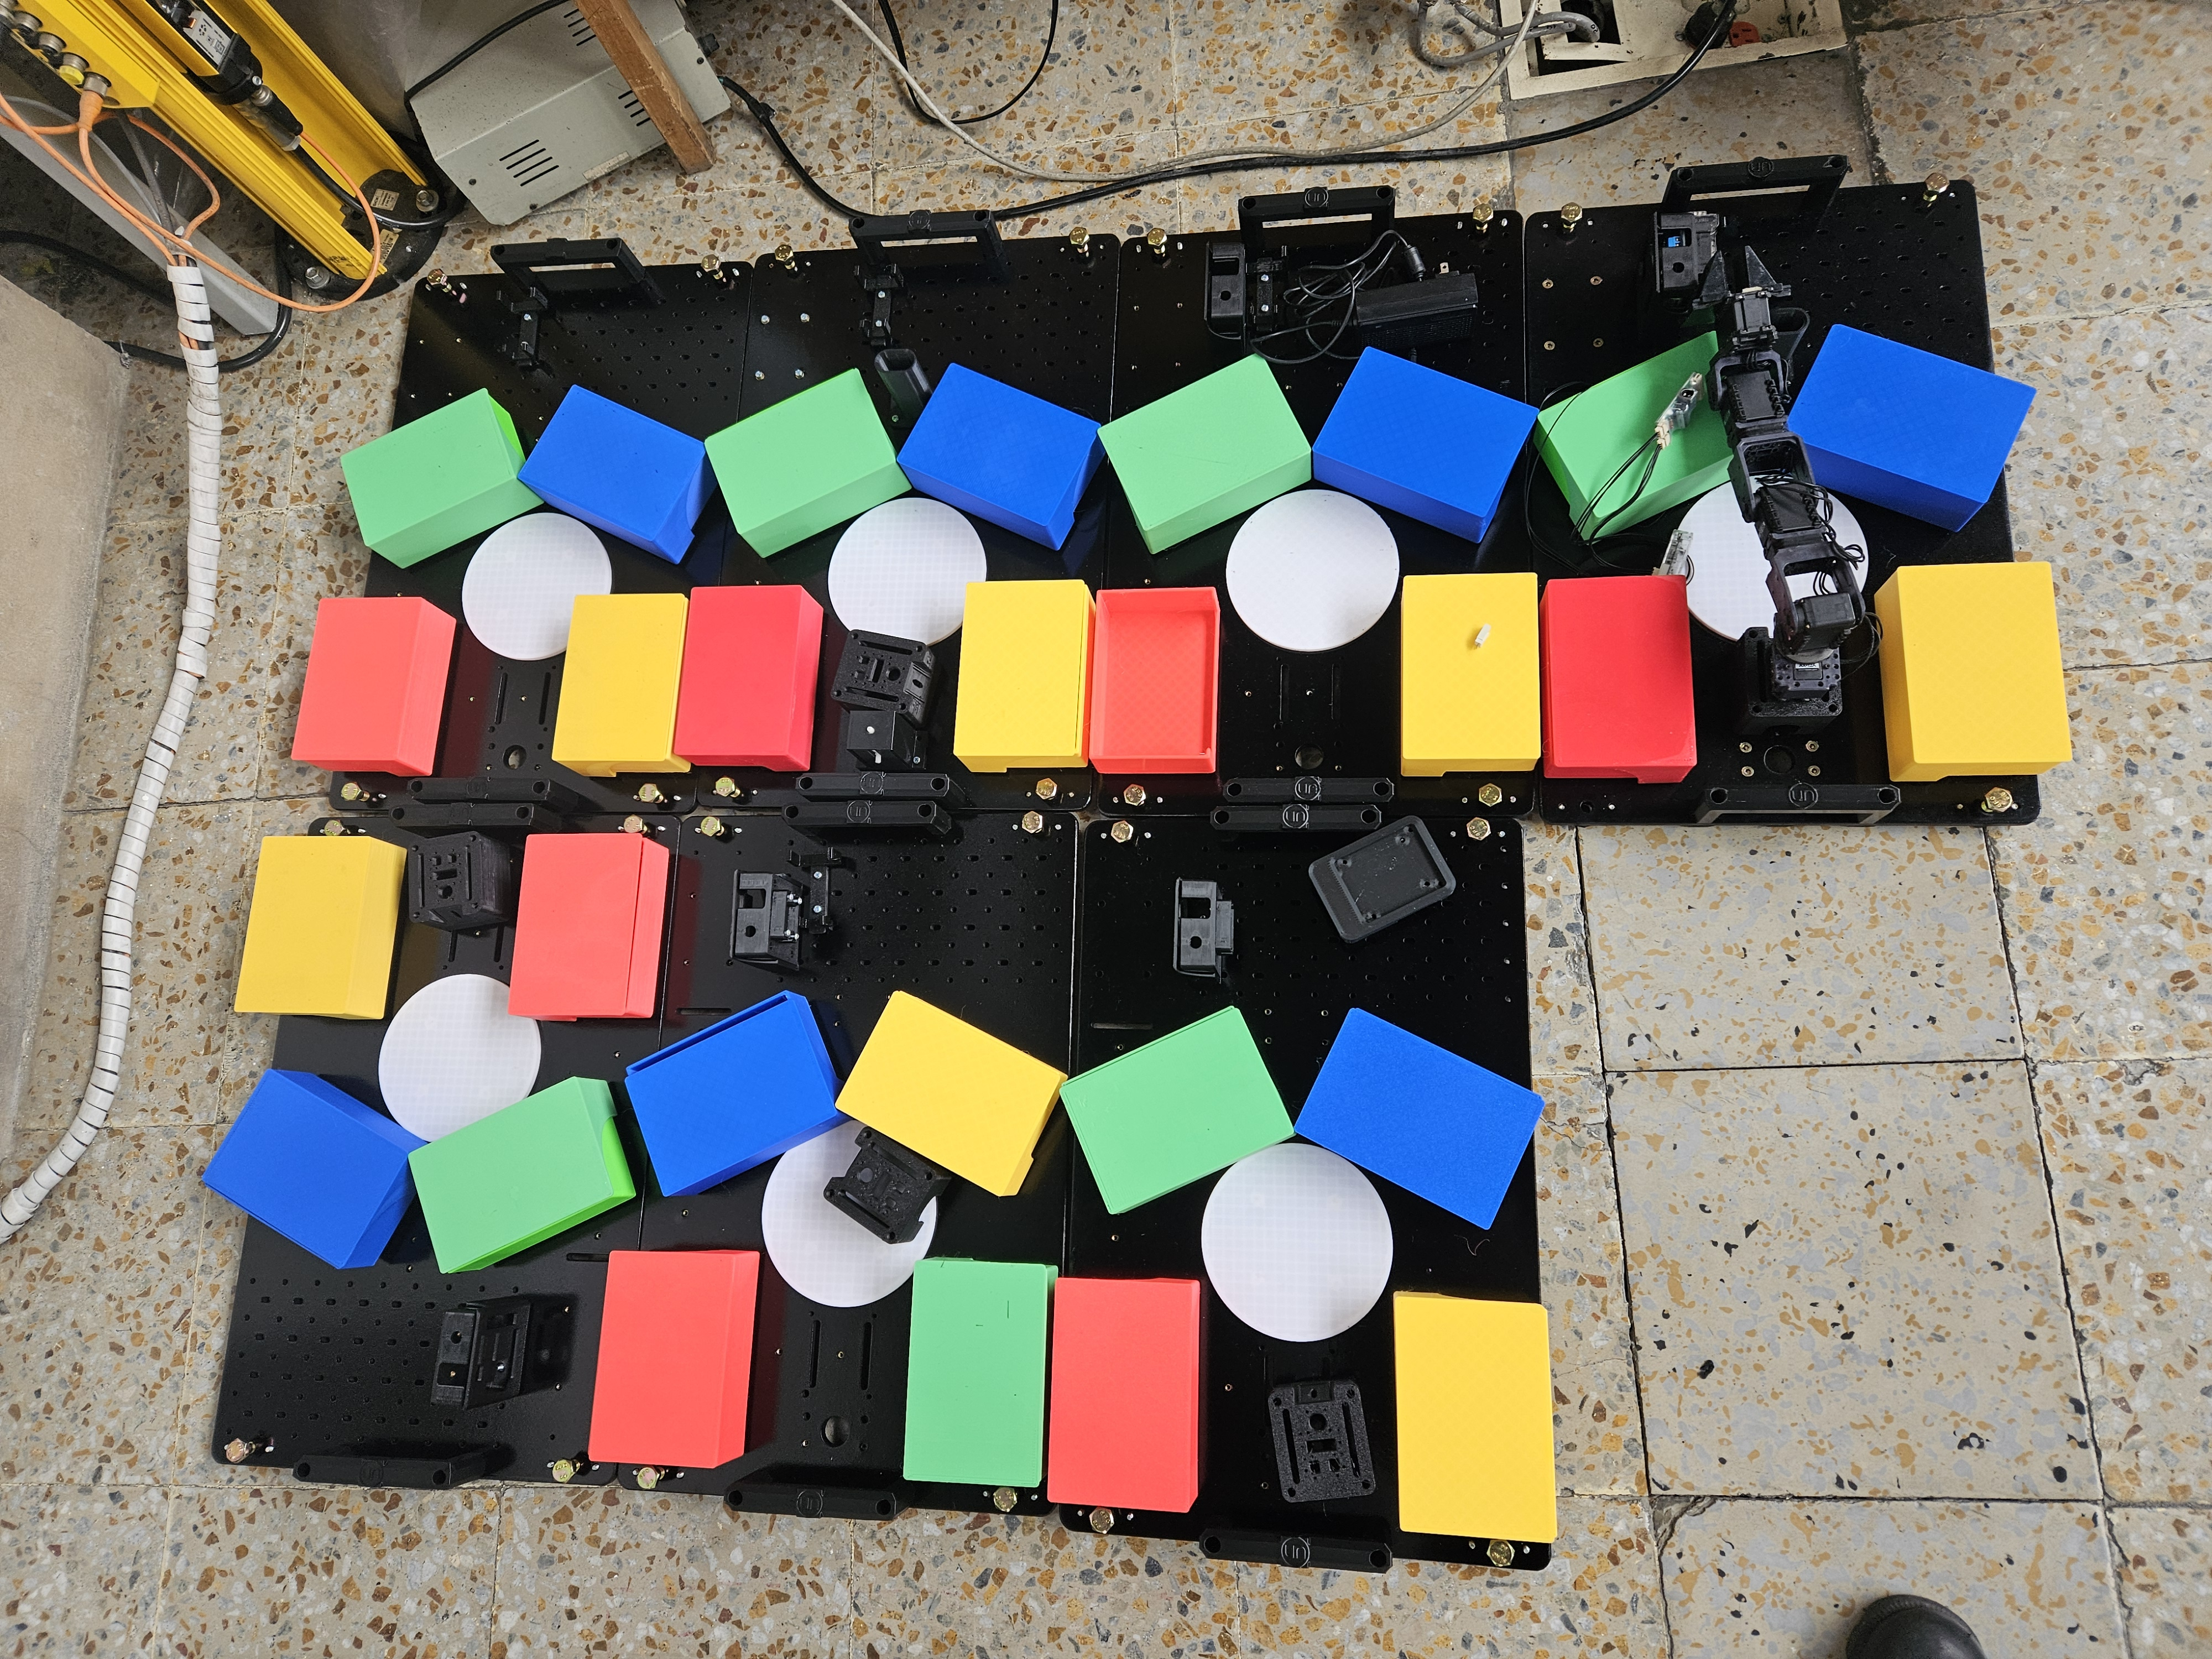
\includegraphics[width=0.95\textwidth]{08prototipo/7kits.jpg}
\caption{Siete kits fabricados para implementación en laboratorio. Vista superior mostrando las plataformas base con acabado negro mate, cuatro zonas de depósito con canecas de colores (roja, amarilla, azul, verde), zonas de recolección circulares blancas, y cinco robots PhantomX Pincher instalados. Dos kits se observan sin robot (extremos), mostrando las bases preparadas para integración posterior.}
\label{fig:siete_kits}
\end{figure}

%==============================================================================
\subsection{Sistema de Almacenamiento}
%==============================================================================

Cada kit se almacena en contenedor plástico industrial tipo canastilla 3/4 (600 × 400 × 171 mm) que permite transporte seguro entre laboratorios. El contenedor incluye protección mediante espuma de polietileno y organización en niveles para componentes del kit.

\begin{figure}[H]
\centering
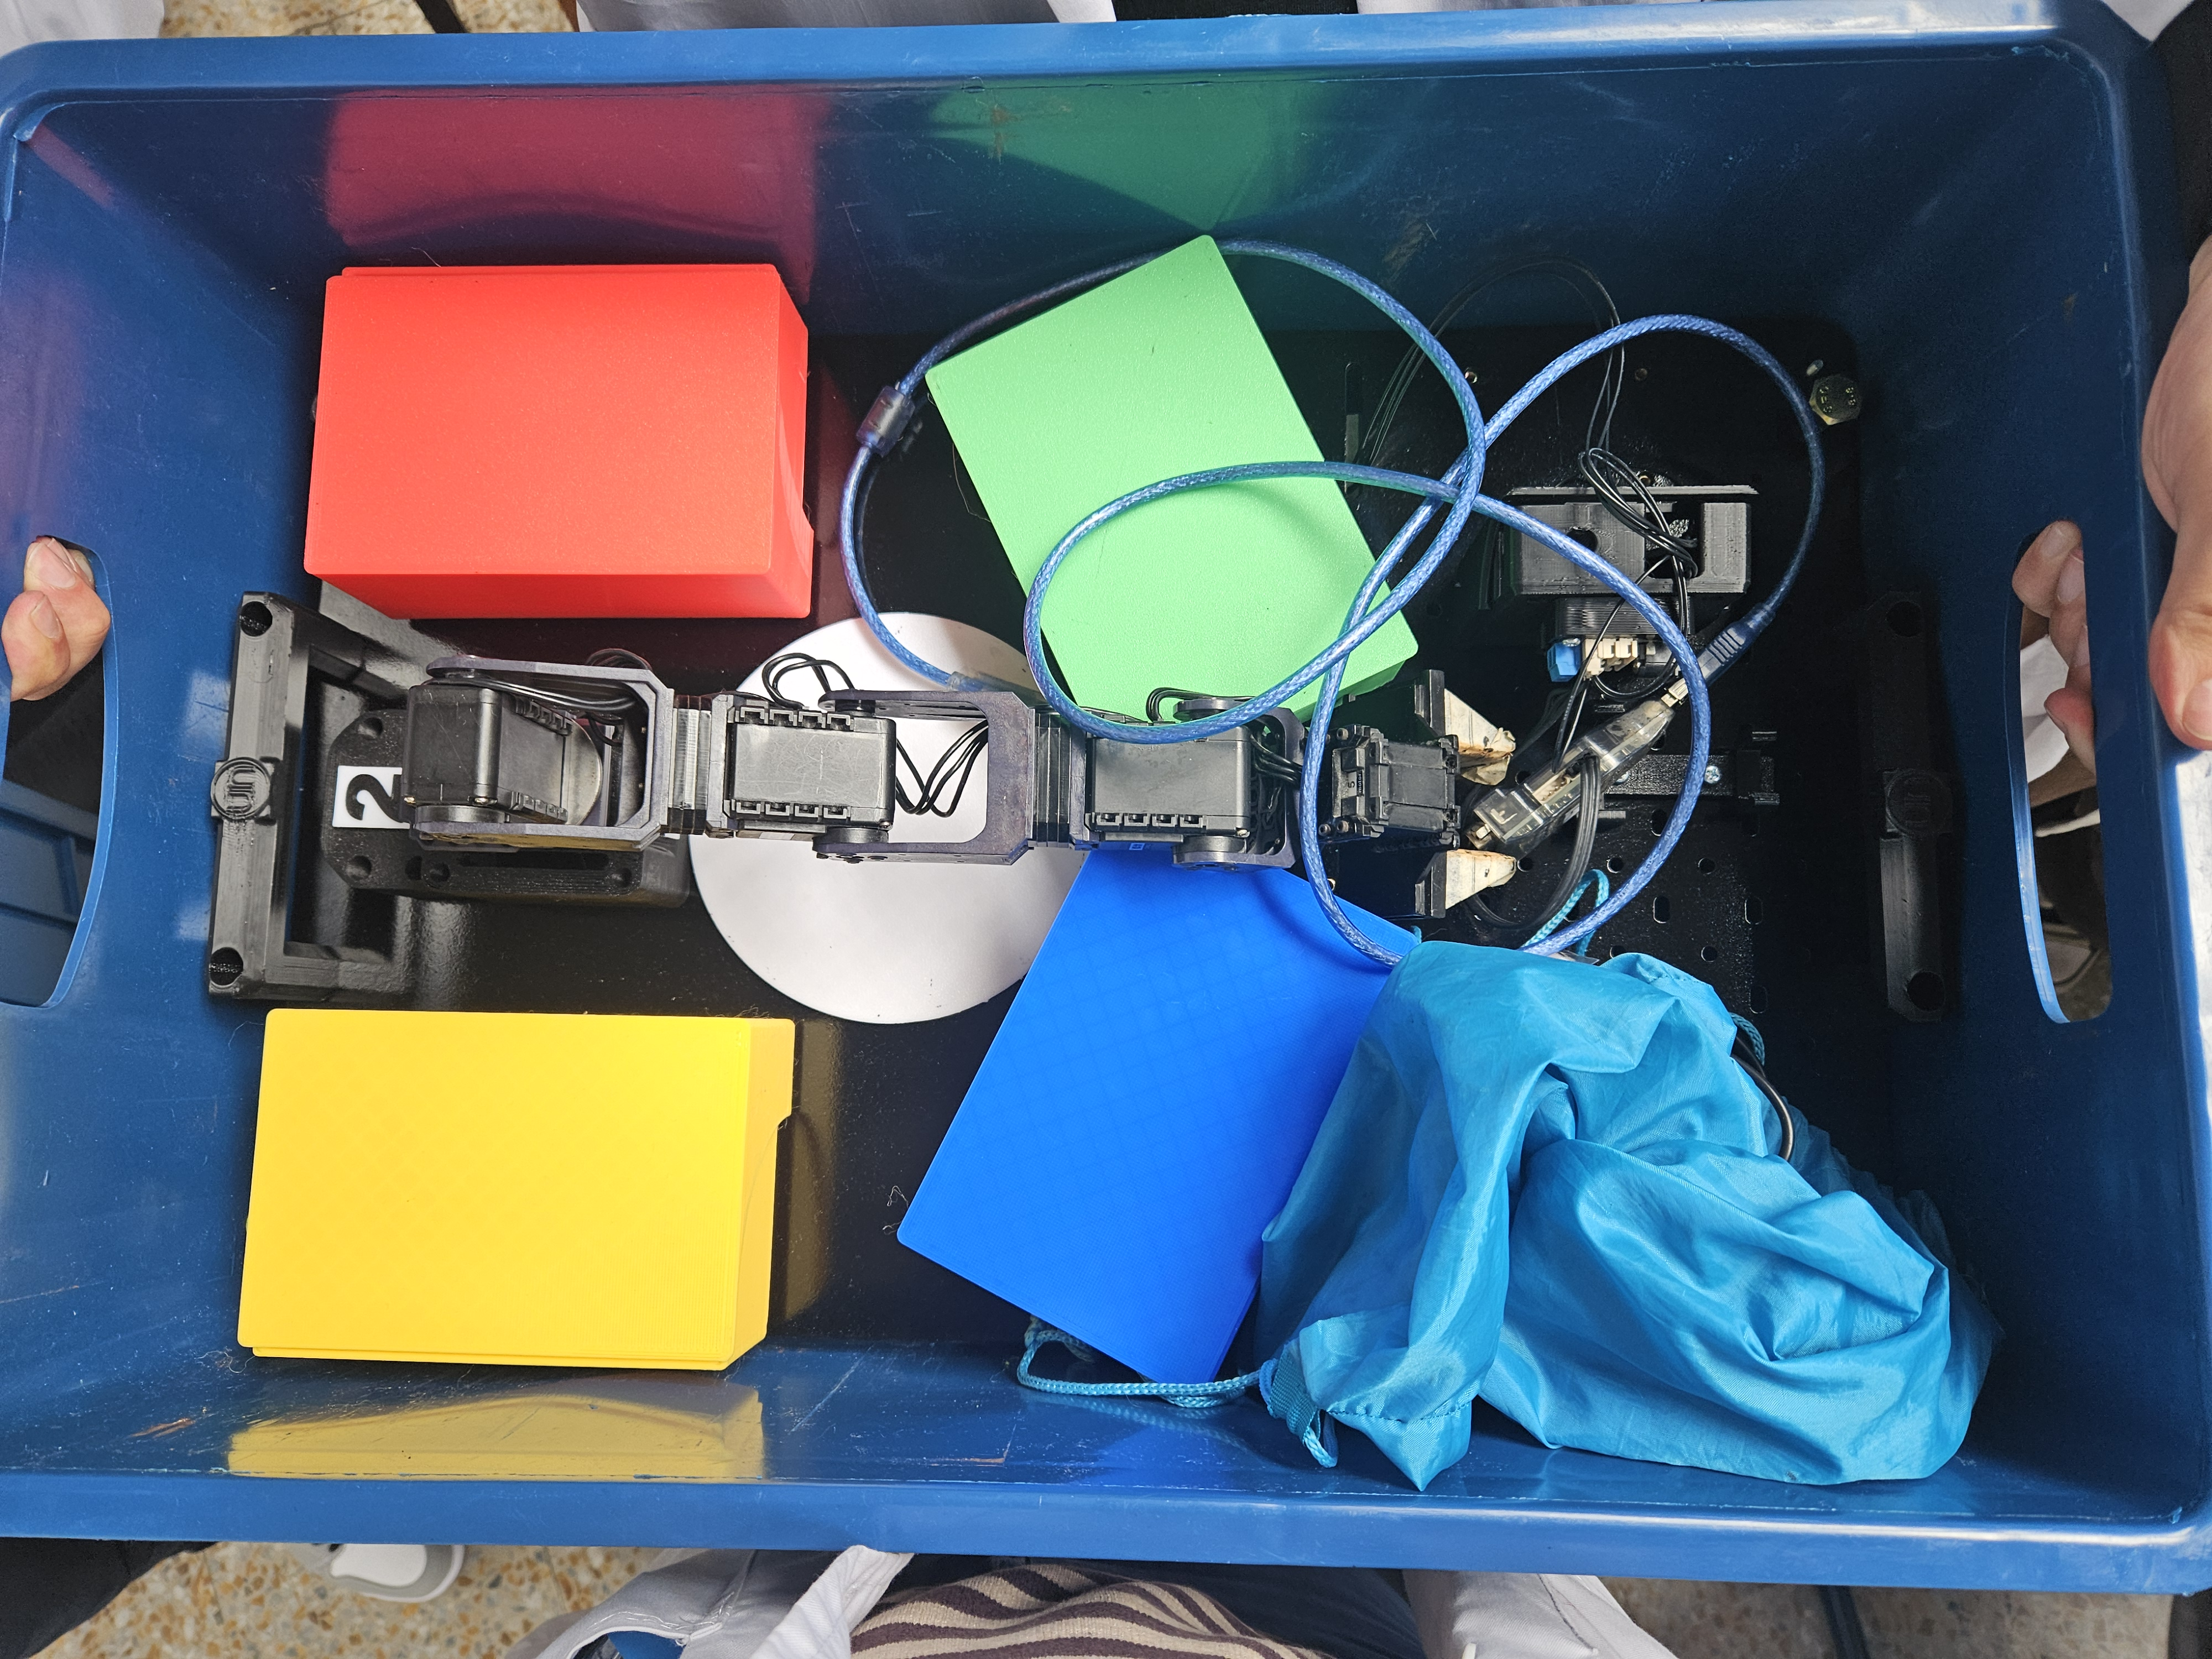
\includegraphics[width=0.75\textwidth]{08prototipo/kitYContenedor.jpg}
\caption{Kit completo en contenedor de transporte. Se observa la plataforma con robot PhantomX Pincher, cuatro canecas con tapas cerradas, zona de recolección circular blanca, y cableado organizado. El contenedor incluye espuma protectora para transporte seguro.}
\label{fig:kit_contenedor}
\end{figure}

%==============================================================================
\subsection{Validación con Estudiantes}
%==============================================================================

Se realizó validación del sistema mediante sesión práctica con estudiantes utilizando los kits en operación real.

\begin{figure}[H]
\centering
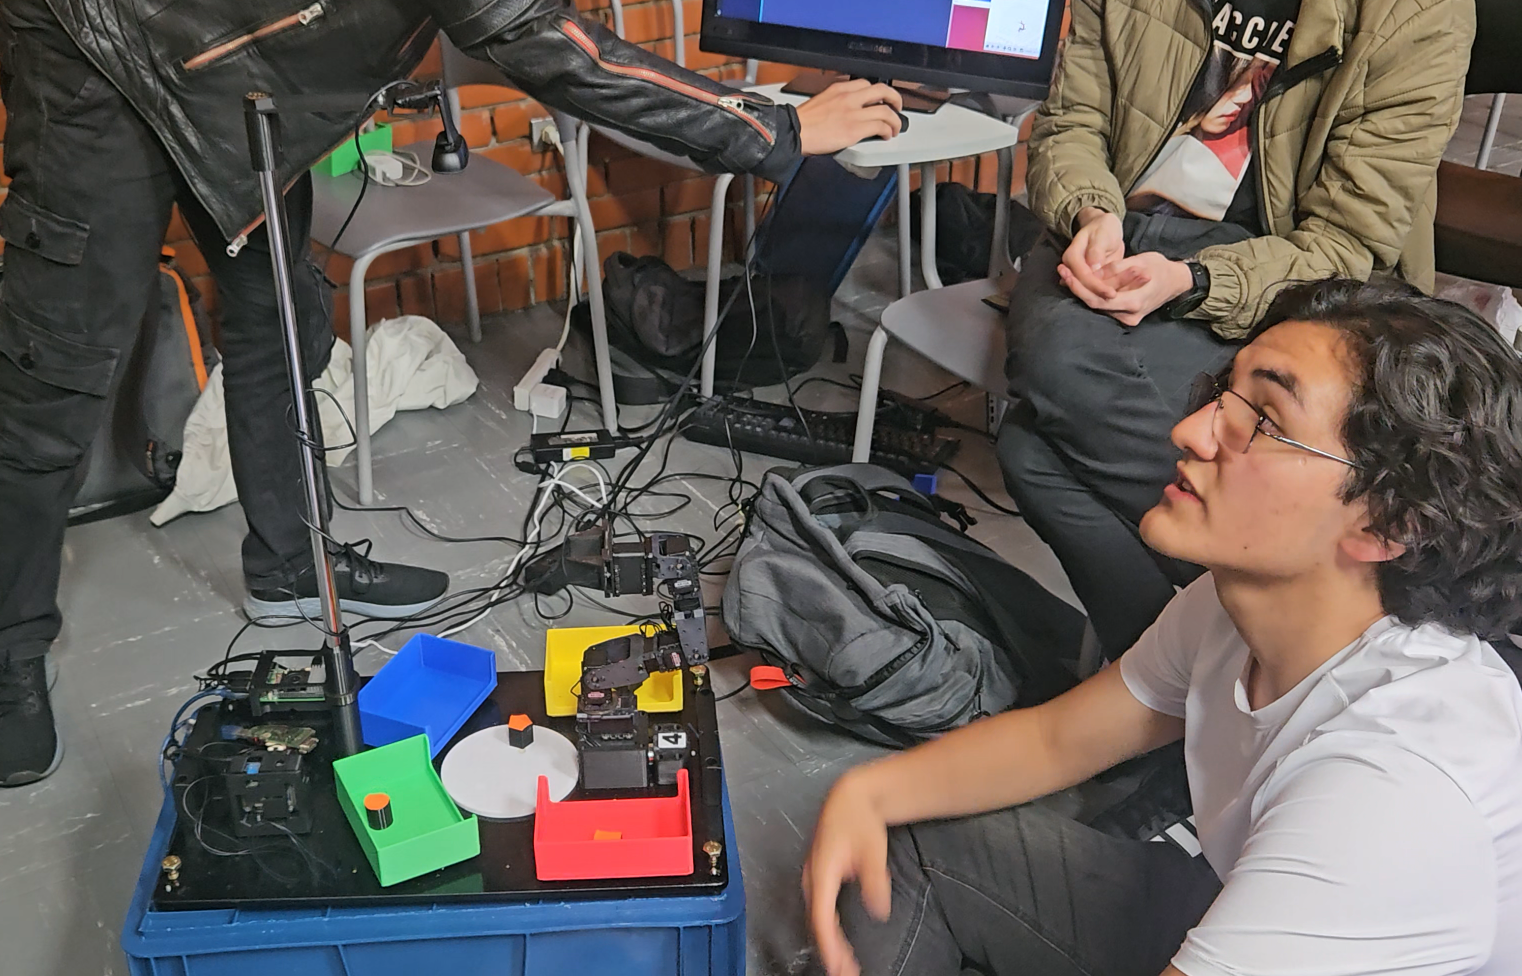
\includegraphics[width=0.9\textwidth]{08prototipo/estudiantesUsandoKiVisionMaquina.png}
\caption{Estudiantes operando el kit en sesión de laboratorio. Se observa el sistema completo en funcionamiento: robot clasificando objetos en las canecas de colores, cámara montada en mástil para captura de imágenes, y estudiantes interactuando con la interfaz de control. La sesión validó la operación integrada de los subsistemas mecánico, electrónico y de visión artificial.}
\label{fig:validacion_estudiantes}
\end{figure}

La construcción de siete kits funcionales demuestra la viabilidad de reproducción del diseño para implementación en entornos educativos.